\pagebreak
\section{Background}
\label{sec:background}
In this section we consider a portion of available literature on both CRs and control to motivate the use of learning-based control for the PCR considered in this work. As learning-based control for a PCR configuration has not yet been studied in the available literature, the scope of this section is only to provide a background of relevant topics and not a comprehensive review of all available control and modelling methods. 


\subsection{Types of Continuum Robots}
CRs can be defined as "an actuatable structure whose constitutive material forms curves with continuous tangent vectors." \cite{7314984} CRs are robots with an infinite number of joints and degrees of freedom. By using flexible components, CRs are inherently compliant, making them useful in applications where interactions with stiff joints may cause damage to the environment. They are also able to be manufactured on sub-millimeter scales. As such, these robots have seen use in medical and inspection applications \cite{7314984, DONG2017218, 4058827}. Continuum robots come in a variety of configurations, materials, and actuation methods \cite{doi:10.34133/2022/9754697}. Modelling methods for continuum robots are discussed in Section \ref{sec:modelling_methods}. The subset of continuum robots pertaining to this thesis is considered.  

\begin{figure}[H]
    \centering
    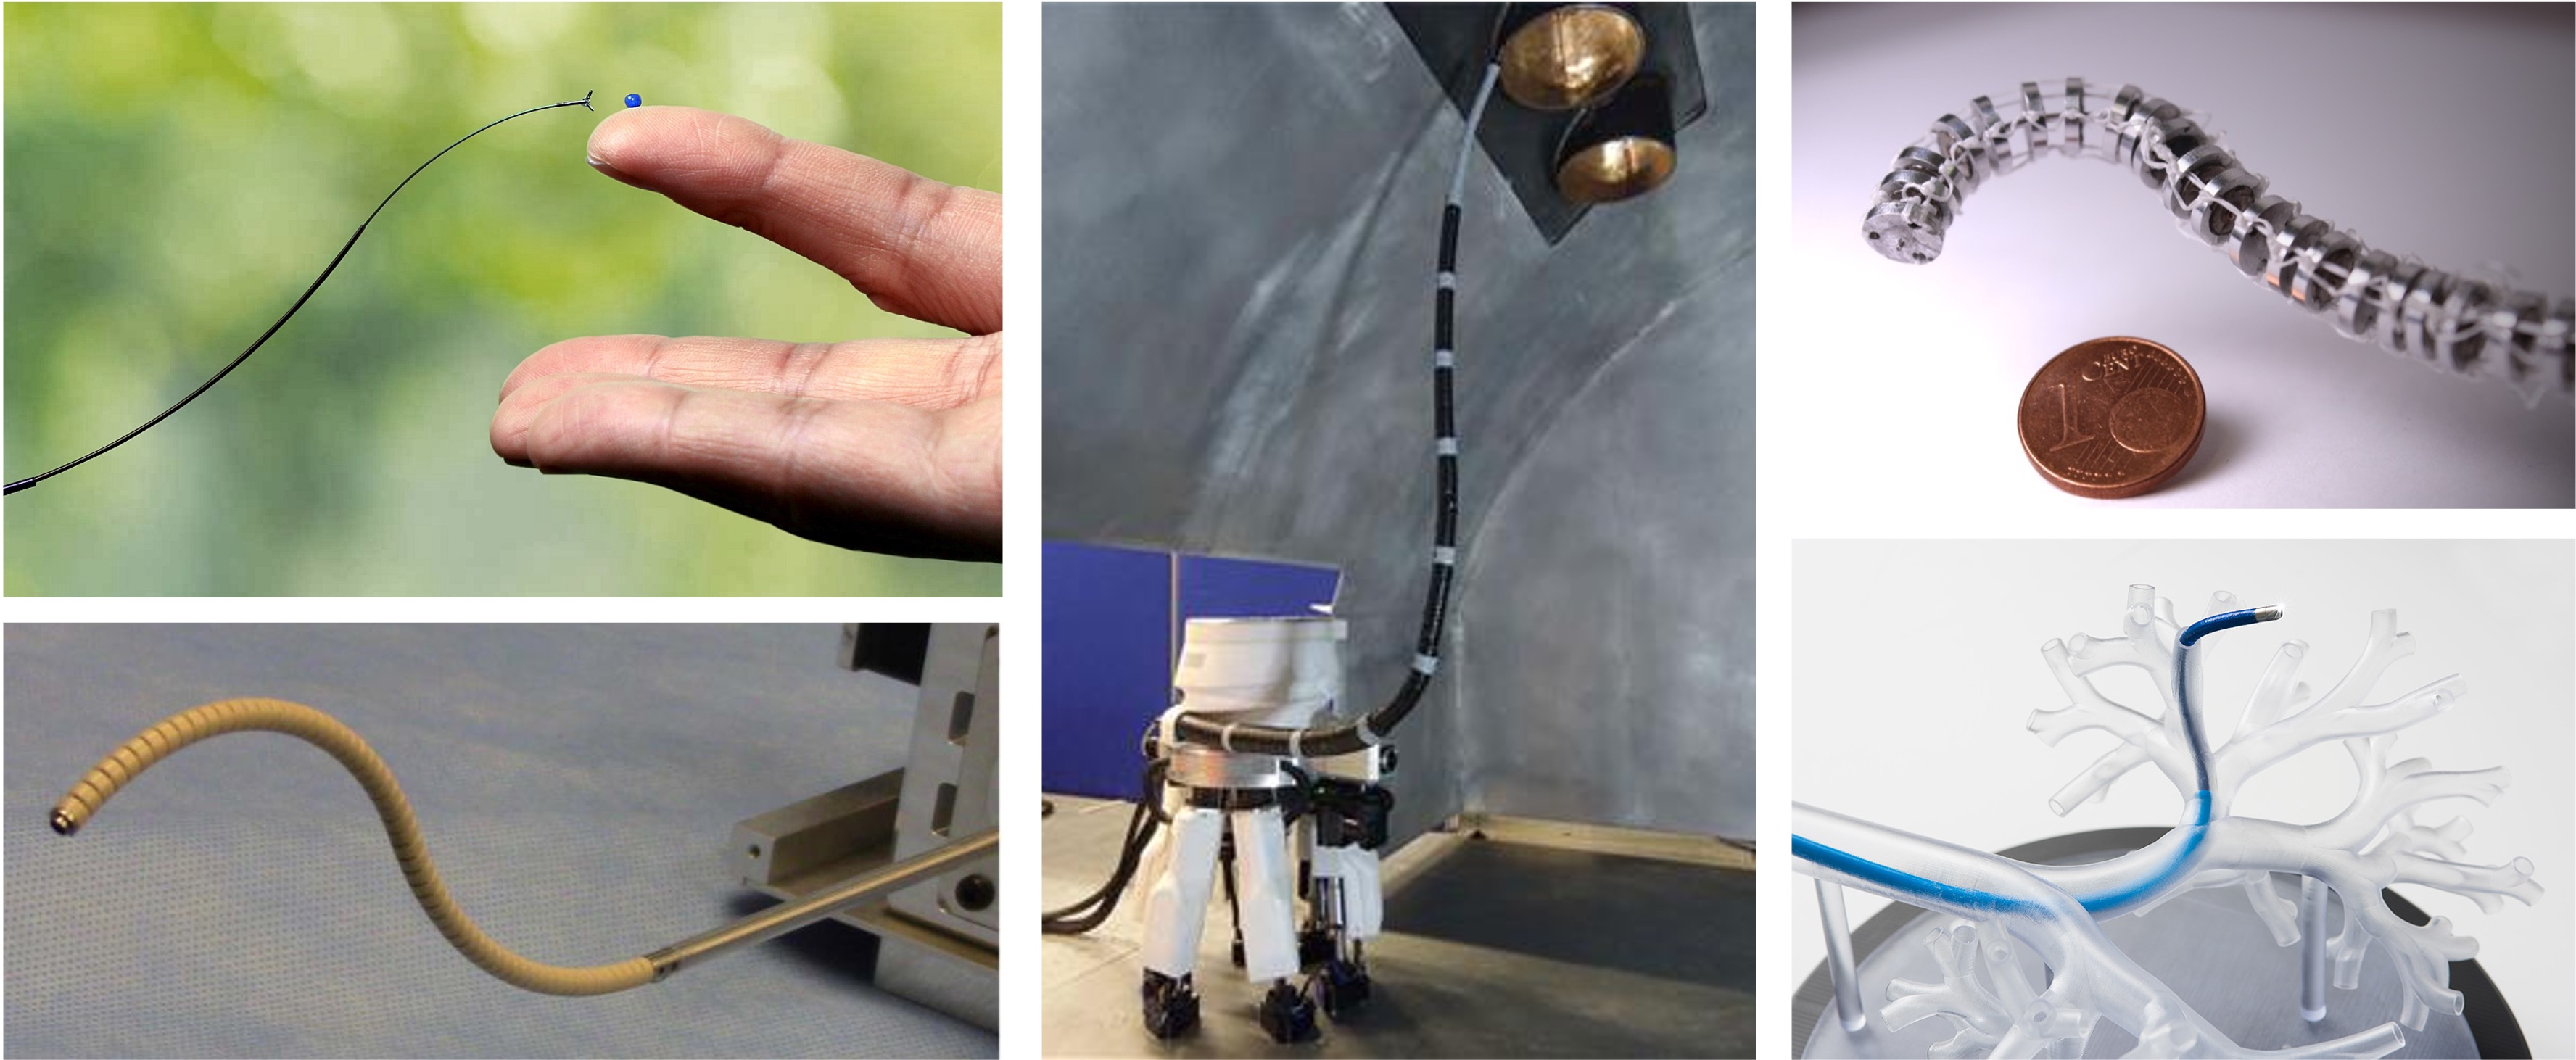
\includegraphics[width=\textwidth]{images/cr_examples.jpg}
    \caption{Continuum robot examples, from \cite{crl_cr_types}}
    \label{fig:cr_examples}
\end{figure}

\subsubsection{Tendon-Driven Continuum Robots}
Tendon-Driven Continuum Robots (TDCR) are a class of CRs that are actuated by contracting a tendon that is attached to a point along the robot's backbone. The backbone is typically a highly elastic rod or beam that provides stiffness to the robot while remaining compliant. The tendon is constrained to be a fixed distance from the backbone by a series of spacer disks. Contracting the tendon results in the backbone bending towards the side the tendon is offset on \cite{HEMAMI198527, 10.3389/frobt.2020.630245}. An "arm" of a TDCR refers to a single beam that can be actuated independently of other arms in the robot. 

\subsubsection{Parallel Continuum Robots}
PCRs use multiple arms joined together to increase the stiffness and maximum applied force of a CR while maintaining the inherent compliance that CRs have to offer \cite{survey}. 

\subsubsection{Robot Configurations}
PCRs can take on a wide variety of configurations. In \cite{6906943}, a six-beam PCR is proposed and modelled based on Cosserat rod theory. Flexible rods are translationally pushed and pulled to achieve actuation. A tracking accuracy of 2.89\% of the length of one arm of the robot was achieved.  \cite{slilge_2020} introduces a three-beam parallel TDCR with six degrees of freedom at the end effector. The authors model each beam using a geometric kinematic model based on the constant curvature assumption. A planar configuration reduces the task space to a 2D plane. These robots have at most three degrees of freedom at the end effector; two spatial components and a rotational one. In \cite{9143427}, a planar PCR is proposed along with a geometric model controller based on the constant curvature assumption. It achieves an accuracy of 1\% of the length of one arm of the robot.  


\subsection{Modelling Continuum Robots}
\label{sec:modelling_methods}
It is desirable to construct a forward and inverse kinematic model when controlling a robot. A forward kinematic model provides an expression for the end effector position given a robot's joint variables. It is used to estimate the end effector position of a robot during operation when direct measurements are not available. An inverse kinematic model solves for a robot's joint variables given a desired end effector position. It is used in control tasks to move the robot into a desired configuration. In both cases, the accuracy of the model is determined by a number of factors including the simplifying assumptions made in exchange for increased computational efficiency \cite{10.3389/frobt.2020.630245}. Figure \ref{fig:timing_from_source} demonstrates the run time benefit from using models that make simplifying assumptions and the sacrifice that is made in terms of accuracy. 

\begin{figure}[h]
    \centering
    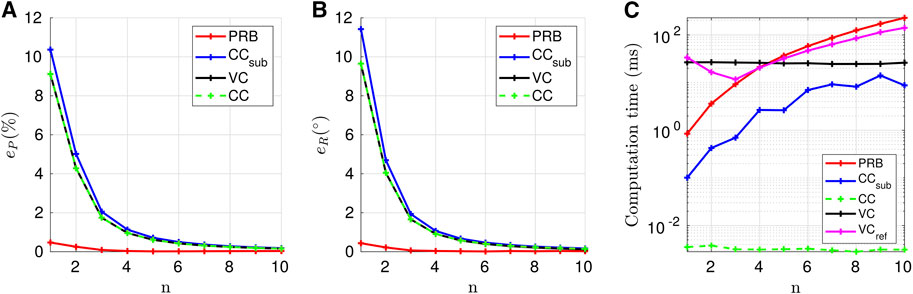
\includegraphics[width=\textwidth]{images/time_graph_from_survey.jpg}
    \caption{Timing analysis of pseudo-rigid body, constant curvature, and variable curvature modelling methods in a simulated environment, from \cite{10.3389/frobt.2020.630245}}
    \label{fig:timing_from_source}
\end{figure}

There are three major types of robot models that we consider: (1) kinematic models, (2) static models, and (3) dynamic models. Kinematic models model the shape of the robot without consideration of forces. Static models consider the robot at points of equilibrium, where the robot is not moving and has zero net force. Dynamic models model the robot as it's moving, accounting for transient effects (such as spring forces, friction, air resistance, etc.). 

In rigid robotics, simple linear models exist that accurately model the robot's motion. CRs do not have such a luxury due to their non-linear deformation. As such, more system assumptions or more complex models must be used for even the simplest of CRs \cite{10.3389/frobt.2020.630245}. As this is an emerging research field, the accuracy of models for CRs is not yet comparable to conventional industrial robots. 

\subsubsection{Constant Curvature Assumption}
The most common and convenient kinematic modelling approach for continuum robots uses the constant curvature (CC) assumption \cite{doi:10.1177/0278364910368147}. It assumes that the curvature throughout the entire length of an arm is constant. This assumption greatly reduces the complexity of the forward and inverse kinematic models of a continuum robot. 

\paragraph{Euler Beam Theory}
Euler beam theory can be used to create a static model assuming that the effects of shear and twist are negligible \cite{10.3389/frobt.2020.630245}. The CC assumption allows for computationally efficient implementations of the inverse kinematics problem. It does however result in a number of inaccuracies as beams under high bending do not have CC. Modelling a continuum robot using the CC assumption and Euler beam theory has been shown to result in poorer accuracy compared to using a variable curvature model \cite{10.3389/frobt.2020.630245}.

\subsubsection{Variable Curvature Representation}
Without losing generality, one can model the curvature of a continuum robot using a variable curvature representation. This representation makes no assumptions about the backbone shape as it can model any point along it with six degrees of freedom \cite{10.3389/frobt.2020.630245}.  

\paragraph{Cosserat Rod Theory}
The Cosserat theory of elastic rods extends the variable curvature kinematic representation into a static model. Modelling in this way accounts for shear deformations, something Euler beam theory did not. While the Cosserat rod theory approach has been shown to produce excellent accuracy in continuum robot applications \cite{10.3389/frobt.2020.630245, CAO2008460, ALQUMSAN201948, 10.1007/978-3-319-64107-2_56}, it does so at great computation costs, resulting in the inability to be used for real-time control \cite{10.3389/frobt.2020.630245, ALQUMSAN201948}. A number of implementations for the cosserat theory model have been realized with accuracies ranging from 12\%\cite{10.1007/978-3-319-64107-2_56} to \SI{4e-10}{m} - \SI{8e-10}{m} Root Mean Squared Error (RMSE) for a robot of length \SI{30}{cm}\cite{ALQUMSAN201948}. 


\subsection{Machine Learning}
Machine learning has emerged as a useful tool for estimating complex functions using data collected from a system. In robotics, learning has been used to develop controllers for complex systems that are difficult to model. Deep learning approaches have shown promise in modelling complex dynamic behaviour for controller design in robotics \cite{9199280}. Because data-driven approaches can estimate arbitrarily complex functions \cite{HORNIK1989359} they are thought to be useful in continuum robots. Learning-based applications in continuum robotics have primarily focused on learning the inverse statics and kinematics of a robot \cite{10.3389/frobt.2021.730330}. With each of the results reviewed here, one must be weary of directly comparing results directly as large variations in performance can arise from changes in robot configuration, actuation type, and construction. In each of the works reviewed, the proposed learning-based model outperformed baseline approaches on the same robot.

\subsubsection{In Continuum Robotics}
\paragraph{Data-driven approaches}
 In \cite{8115276}, the authors use a model-free approach using an adaptive Kalman Filter. This uses sensor data to update the model's uncertainty estimations during operation, resulting in a more controller that had an experimental tracking RMSE of \SI{1.52}{mm} (with a \SI{20}{cm} - \SI{25}{cm} long pneumatic continuum robot). In \cite{rcs.1774}, the authors implement three regression models to learn the inverse kinematics of a flexible surgical robot, achieving a top RMSE of \SI{2.1275}{mm} with a KNN regression. The authors do not report the total robot length. 

\paragraph{Deep learning approaches}
For deep learning approaches to work, a large amount of data or an accurate simulation environment must be available. As the dynamic effects of a continuum robot are what is difficult to model, simulation environments are not readily available. In \cite{grassmann2022a}, a dataset is released for concentric tube continuum robots. The authors propose a baseline learning model that achieves tip tracking errors of \SI{0.74}{mm} (or 0.4\% of the robot's length).  Using deep neural networks for approximating the inverse statics equation is the approach used in \cite{7112506}. The authors are able to achieve errors of around \SI{7}{mm}\footnote{Number, as reported, is an estimation by the thesis author. See reference paper for complete results breakdown.} for an underwater soft continuum robot (or about 2.5\% of the robot's length). For both of these implementations, a large amount of data is required that maps the robot's end effector position to its joint configuration, marking a large drawback to deep learning-based models. 

\subsubsection{In Other Robotics}
Although learning-based solutions are limited in their applications to CRs, they have been deeply explored in other robotics in areas that may be applicable to CRs such as sensing \cite{8643440, 9001195}, state estimation \cite{s21062085, 8972568, 8643440}, and control \cite{doi:10.1146/annurev-control-090419-075625, TOQUICA2021106682}. Each of these aspects have had results that demonstrate learning-based solutions and their ability to replace more conventional methods. Often however, hybrid approaches that make use of conventional modelling methods that are augmented using learning are shown to have the best results. 

In \cite{s21062085}, the authors highlight several elements in deep learning that prove useful in state estimation including the use of long short-term memory (LSTM) layers to enable long-term correspondence between input data, the use of Bayesian modelling to help account for complex system noise, and applying attention mechanisms to learn what is important and unimportant in the input data at each time step. The survey goes on to highlight the value in hybrid approaches that integrate learned systems with model-based approaches. The authors in \cite{8972568} take this one step further by demonstrating the hybrid approach on a manipulation task with a deformable object. The authors show that they can accurately estimate a rope's full state using a self-supervised deep learning network trained on image data. 

Robotic systems rely on their sensor data as the basis for state estimation. This data is generally corrupted by some amount of noise. \cite{8643440} demonstrates the use of deep learning to explicitly account for system noise in attitude estimation of a UAV. The authors in \cite{9001195} propose a pipeline for explicit handling of uncertainty caused from noisy inputs. They demonstrate their approach's success in robotic applications by estimating model uncertainty by propagating noise through the model and quantifying the effect. 

For learning-based control, \cite{doi:10.1146/annurev-control-090419-075625} highlights how neural networks can improve results in model predictive control (MPC). It looks at three different applications including using learning to model system dynamics and using learning to enhance objective function design. In \cite{TOQUICA2021106682}, deep learning is used to solve the inverse kinematic problem for a rigid parallel industrial robot. The work shows that deep learning based inverse kinematic solutions have applications in parallel robotics, boasting a 99.8\% accuracy compared to the analytical model. 


\subsection{Summary}
PCR design is still an open area of research. Work has focused on the benefits of these robots in their relevant application spaces. Research modelling and control for CRs have largely focused on single-beam CRs. A research gap exists for modelling and control of PCRs that is unaddressed by current classical modelling methods. Significant modelling assumptions that ignore dynamic effects of the system or make inaccurate claims about the kinematic description of the system allow for fast but inaccurate control. When these assumptions are not made, controllers have infeasible computation speeds for real-time control. Data-driven approaches may be able to solve this problem but are underdeveloped for parallel continuum robots. This thesis aims to address this gap by taking steps towards learning-based control for a planar parallel TDCR. 